\section{Theorie- und Prüfungsfragen}


\begin{enumerate}
\itemsep1pt\parskip0pt\parsep0pt
\item[1] Skizziere die Schaltung eines Reihenschwingkreises.
\item[2] Skizziere die Schaltung eines Parallelschwingkreises.
\item[3] Was ist die Resonanzfrequenz und wie lässt sie sich berechnen?
\item[4] Berechne die theoretische Resonanzfrequenz der Schwingkreise bei Verwendung eines $50\Omega$ Widerstandes, eines $10pF$ Kondensators und einer Spule mit $270H$.
\end{enumerate}



\begin{enumerate}
\item[5] \emph{\textbf{TD204}}    Wie ändert sich die Resonanzfrequenz eines Schwingkreises, wenn 1. die Spule weniger Windungen erhält, 2. die Länge der Spule durch Zusammenschieben der Drahtwicklung verringert wird, 3. ein Ferritkern in das Innere der Spule gebracht wird? 
	\begin{enumerate}
	\itemsep1pt\parskip0pt\parsep0pt
		\item[a] Die Resonanzfrequenz wird bei 1. und 2. kleiner und bei 3. größer. 
		\item[b] Die Resonanzfrequenz wird bei 1. kleiner und bei 2. und 3. größer.
		\item[c] Die Resonanzfrequenz wird bei 1. und 2. größer und bei 3. kleiner.
		\item[d] Die Resonanzfrequenz wird bei 1. größer und bei 2. und 3. kleiner. 
	\end{enumerate}
\end{enumerate}


\loesung{
	\begin{figure}[H]
	\center
	% Graphic for TeX using PGF
% Title: /media/sda2/owncloud_tu.berlin/Dia/Reihenschwingkreis.dia
% Creator: Dia v0.97.3
% CreationDate: Thu Nov 12 20:47:37 2015
% For: stole
% \usepackage{tikz}
% The following commands are not supported in PSTricks at present
% We define them conditionally, so when they are implemented,
% this pgf file will use them.
\ifx\du\undefined
  \newlength{\du}
\fi
\setlength{\du}{15\unitlength}
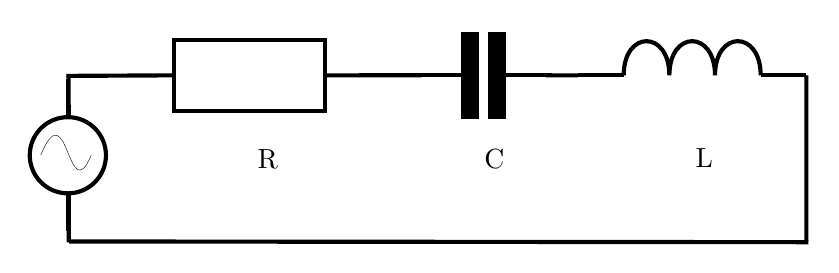
\begin{tikzpicture}
\pgftransformxscale{1.000000}
\pgftransformyscale{-1.000000}
\definecolor{dialinecolor}{rgb}{0.000000, 0.000000, 0.000000}
\pgfsetstrokecolor{dialinecolor}
\definecolor{dialinecolor}{rgb}{1.000000, 1.000000, 1.000000}
\pgfsetfillcolor{dialinecolor}
\pgfsetlinewidth{0.100000\du}
\pgfsetdash{}{0pt}
\pgfsetdash{}{0pt}
\pgfsetbuttcap
\pgfsetmiterjoin
\pgfsetlinewidth{0.100000\du}
\pgfsetbuttcap
\pgfsetmiterjoin
\pgfsetdash{}{0pt}
\definecolor{dialinecolor}{rgb}{0.000000, 0.000000, 0.000000}
\pgfsetfillcolor{dialinecolor}
\fill (17.992700\du,8.993760\du)--(17.992700\du,10.993760\du)--(18.326033\du,10.993760\du)--(18.326033\du,8.993760\du)--cycle;
\definecolor{dialinecolor}{rgb}{0.000000, 0.000000, 0.000000}
\pgfsetstrokecolor{dialinecolor}
\draw (17.992700\du,8.993760\du)--(17.992700\du,10.993760\du)--(18.326033\du,10.993760\du)--(18.326033\du,8.993760\du)--cycle;
\pgfsetbuttcap
\pgfsetmiterjoin
\pgfsetdash{}{0pt}
\definecolor{dialinecolor}{rgb}{0.000000, 0.000000, 0.000000}
\pgfsetfillcolor{dialinecolor}
\fill (18.659367\du,8.993760\du)--(18.659367\du,10.993760\du)--(18.992700\du,10.993760\du)--(18.992700\du,8.993760\du)--cycle;
\definecolor{dialinecolor}{rgb}{0.000000, 0.000000, 0.000000}
\pgfsetstrokecolor{dialinecolor}
\draw (18.659367\du,8.993760\du)--(18.659367\du,10.993760\du)--(18.992700\du,10.993760\du)--(18.992700\du,8.993760\du)--cycle;
\pgfsetbuttcap
\pgfsetmiterjoin
\pgfsetdash{}{0pt}
\definecolor{dialinecolor}{rgb}{0.000000, 0.000000, 0.000000}
\pgfsetstrokecolor{dialinecolor}
\draw (17.992700\du,9.993760\du)--(16.992700\du,9.993760\du);
\pgfsetbuttcap
\pgfsetmiterjoin
\pgfsetdash{}{0pt}
\definecolor{dialinecolor}{rgb}{0.000000, 0.000000, 0.000000}
\pgfsetstrokecolor{dialinecolor}
\draw (18.992700\du,9.993760\du)--(19.992700\du,9.993760\du);
\pgfsetlinewidth{0.100000\du}
\pgfsetdash{}{0pt}
\pgfsetdash{}{0pt}
\pgfsetmiterjoin
\definecolor{dialinecolor}{rgb}{1.000000, 1.000000, 1.000000}
\pgfsetfillcolor{dialinecolor}
\fill (11.046000\du,9.143310\du)--(11.046000\du,10.845869\du)--(14.680696\du,10.845869\du)--(14.680696\du,9.143310\du)--cycle;
\definecolor{dialinecolor}{rgb}{0.000000, 0.000000, 0.000000}
\pgfsetstrokecolor{dialinecolor}
\draw (11.046000\du,9.143310\du)--(11.046000\du,10.845869\du)--(14.680696\du,10.845869\du)--(14.680696\du,9.143310\du)--cycle;
\pgfsetlinewidth{0.100000\du}
\pgfsetdash{}{0pt}
\pgfsetdash{}{0pt}
\pgfsetbuttcap
\pgfsetmiterjoin
\pgfsetlinewidth{0.100000\du}
\pgfsetbuttcap
\pgfsetmiterjoin
\pgfsetdash{}{0pt}
\definecolor{dialinecolor}{rgb}{0.000000, 0.000000, 0.000000}
\pgfsetstrokecolor{dialinecolor}
\pgfpathmoveto{\pgfpoint{21.869400\du}{9.996500\du}}
\pgfpathcurveto{\pgfpoint{21.869400\du}{8.896500\du}}{\pgfpoint{22.969400\du}{8.896500\du}}{\pgfpoint{22.969400\du}{9.996500\du}}
\pgfpathcurveto{\pgfpoint{22.969400\du}{8.896500\du}}{\pgfpoint{24.069400\du}{8.896500\du}}{\pgfpoint{24.069400\du}{9.996500\du}}
\pgfpathcurveto{\pgfpoint{24.069400\du}{8.896500\du}}{\pgfpoint{25.169400\du}{8.896500\du}}{\pgfpoint{25.169400\du}{9.996500\du}}
\pgfusepath{stroke}
\pgfsetbuttcap
\pgfsetmiterjoin
\pgfsetdash{}{0pt}
\definecolor{dialinecolor}{rgb}{0.000000, 0.000000, 0.000000}
\pgfsetstrokecolor{dialinecolor}
\draw (20.769400\du,9.996500\du)--(21.869400\du,9.996500\du);
\pgfsetbuttcap
\pgfsetmiterjoin
\pgfsetdash{}{0pt}
\definecolor{dialinecolor}{rgb}{0.000000, 0.000000, 0.000000}
\pgfsetstrokecolor{dialinecolor}
\draw (25.169400\du,9.996500\du)--(26.269400\du,9.996500\du);
\pgfsetlinewidth{0.100000\du}
\pgfsetdash{}{0pt}
\pgfsetdash{}{0pt}
\pgfsetbuttcap
{
\definecolor{dialinecolor}{rgb}{0.000000, 0.000000, 0.000000}
\pgfsetfillcolor{dialinecolor}
% was here!!!
\definecolor{dialinecolor}{rgb}{0.000000, 0.000000, 0.000000}
\pgfsetstrokecolor{dialinecolor}
\draw (8.444162\du,10.007780\du)--(11.046000\du,9.994590\du);
}
\pgfsetlinewidth{0.100000\du}
\pgfsetdash{}{0pt}
\pgfsetdash{}{0pt}
\pgfsetbuttcap
{
\definecolor{dialinecolor}{rgb}{0.000000, 0.000000, 0.000000}
\pgfsetfillcolor{dialinecolor}
% was here!!!
\definecolor{dialinecolor}{rgb}{0.000000, 0.000000, 0.000000}
\pgfsetstrokecolor{dialinecolor}
\draw (14.680700\du,9.994590\du)--(16.992700\du,9.993760\du);
}
\pgfsetlinewidth{0.100000\du}
\pgfsetdash{}{0pt}
\pgfsetdash{}{0pt}
\pgfsetbuttcap
{
\definecolor{dialinecolor}{rgb}{0.000000, 0.000000, 0.000000}
\pgfsetfillcolor{dialinecolor}
% was here!!!
\definecolor{dialinecolor}{rgb}{0.000000, 0.000000, 0.000000}
\pgfsetstrokecolor{dialinecolor}
\draw (19.992700\du,9.993760\du)--(20.769400\du,9.996500\du);
}
\pgfsetlinewidth{0.100000\du}
\pgfsetdash{}{0pt}
\pgfsetdash{}{0pt}
\pgfsetbuttcap
{
\definecolor{dialinecolor}{rgb}{0.000000, 0.000000, 0.000000}
\pgfsetfillcolor{dialinecolor}
% was here!!!
\definecolor{dialinecolor}{rgb}{0.000000, 0.000000, 0.000000}
\pgfsetstrokecolor{dialinecolor}
\draw (8.498636\du,9.979275\du)--(8.501166\du,14.018575\du);
}
\pgfsetlinewidth{0.100000\du}
\pgfsetdash{}{0pt}
\pgfsetdash{}{0pt}
\pgfsetbuttcap
{
\definecolor{dialinecolor}{rgb}{0.000000, 0.000000, 0.000000}
\pgfsetfillcolor{dialinecolor}
% was here!!!
\definecolor{dialinecolor}{rgb}{0.000000, 0.000000, 0.000000}
\pgfsetstrokecolor{dialinecolor}
\draw (8.512937\du,13.996732\du)--(26.315800\du,14.013900\du);
}
\pgfsetlinewidth{0.100000\du}
\pgfsetdash{}{0pt}
\pgfsetdash{}{0pt}
\pgfsetbuttcap
{
\definecolor{dialinecolor}{rgb}{0.000000, 0.000000, 0.000000}
\pgfsetfillcolor{dialinecolor}
% was here!!!
\definecolor{dialinecolor}{rgb}{0.000000, 0.000000, 0.000000}
\pgfsetstrokecolor{dialinecolor}
\draw (26.269400\du,9.996500\du)--(26.271000\du,13.990700\du);
}
% setfont left to latex
\definecolor{dialinecolor}{rgb}{0.000000, 0.000000, 0.000000}
\pgfsetstrokecolor{dialinecolor}
\node[anchor=west] at (12.778000\du,12.008200\du){R};
% setfont left to latex
\definecolor{dialinecolor}{rgb}{0.000000, 0.000000, 0.000000}
\pgfsetstrokecolor{dialinecolor}
\node[anchor=west] at (18.239900\du,12.008200\du){C};
% setfont left to latex
\definecolor{dialinecolor}{rgb}{0.000000, 0.000000, 0.000000}
\pgfsetstrokecolor{dialinecolor}
\node[anchor=west] at (23.332000\du,11.989400\du){L};
\pgfsetlinewidth{0.100000\du}
\pgfsetdash{}{0pt}
\pgfsetdash{}{0pt}
\pgfsetbuttcap
\pgfsetmiterjoin
\pgfsetlinewidth{0.100000\du}
\pgfsetbuttcap
\pgfsetmiterjoin
\pgfsetdash{}{0pt}
\definecolor{dialinecolor}{rgb}{1.000000, 1.000000, 1.000000}
\pgfsetfillcolor{dialinecolor}
\pgfpathellipse{\pgfpoint{8.479509\du}{11.919697\du}}{\pgfpoint{0.917979\du}{0\du}}{\pgfpoint{0\du}{0.917979\du}}
\pgfusepath{fill}
\definecolor{dialinecolor}{rgb}{0.000000, 0.000000, 0.000000}
\pgfsetstrokecolor{dialinecolor}
\pgfpathellipse{\pgfpoint{8.479509\du}{11.919697\du}}{\pgfpoint{0.917979\du}{0\du}}{\pgfpoint{0\du}{0.917979\du}}
\pgfusepath{stroke}
\pgfsetbuttcap
\pgfsetmiterjoin
\pgfsetdash{}{0pt}
\definecolor{dialinecolor}{rgb}{0.000000, 0.000000, 0.000000}
\pgfsetstrokecolor{dialinecolor}
\draw (8.479509\du,11.001718\du)--(8.479509\du,10.083738\du);
\pgfsetlinewidth{0.010000\du}
\pgfsetbuttcap
\pgfsetmiterjoin
\pgfsetdash{}{0pt}
\definecolor{dialinecolor}{rgb}{0.000000, 0.000000, 0.000000}
\pgfsetstrokecolor{dialinecolor}
\pgfpathmoveto{\pgfpoint{7.825448\du}{11.919697\du}}
\pgfpathcurveto{\pgfpoint{8.479509\du}{10.336183\du}}{\pgfpoint{8.479509\du}{13.250767\du}}{\pgfpoint{9.041771\du}{11.919697\du}}
\pgfusepath{stroke}
\pgfsetlinewidth{0.100000\du}
\pgfsetbuttcap
\pgfsetmiterjoin
\pgfsetdash{}{0pt}
\definecolor{dialinecolor}{rgb}{0.000000, 0.000000, 0.000000}
\pgfsetstrokecolor{dialinecolor}
\draw (8.479509\du,12.837677\du)--(8.479509\du,13.755656\du);
\end{tikzpicture}
\\
	\caption{1 Reihenschwingkreis}
	\end{figure}
	
	\begin{figure}[H]
	\center
	% Graphic for TeX using PGF
% Title: /media/sda2/owncloud_tu.berlin/Dia/Parallelschwingkreis.dia
% Creator: Dia v0.97.3
% CreationDate: Thu Nov 12 20:44:59 2015
% For: stole
% \usepackage{tikz}
% The following commands are not supported in PSTricks at present
% We define them conditionally, so when they are implemented,
% this pgf file will use them.
\ifx\du\undefined
  \newlength{\du}
\fi
\setlength{\du}{15\unitlength}
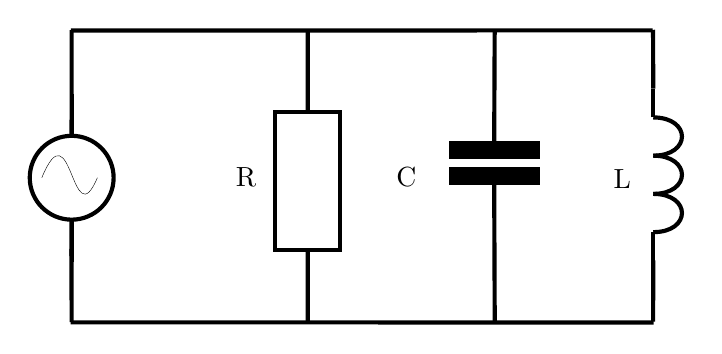
\begin{tikzpicture}
\pgftransformxscale{1.000000}
\pgftransformyscale{-1.000000}
\definecolor{dialinecolor}{rgb}{0.000000, 0.000000, 0.000000}
\pgfsetstrokecolor{dialinecolor}
\definecolor{dialinecolor}{rgb}{1.000000, 1.000000, 1.000000}
\pgfsetfillcolor{dialinecolor}
\pgfsetlinewidth{0.100000\du}
\pgfsetdash{}{0pt}
\pgfsetdash{}{0pt}
\pgfsetmiterjoin
\definecolor{dialinecolor}{rgb}{1.000000, 1.000000, 1.000000}
\pgfsetfillcolor{dialinecolor}
\fill (8.949410\du,11.975600\du)--(8.949410\du,15.298966\du)--(10.521227\du,15.298966\du)--(10.521227\du,11.975600\du)--cycle;
\definecolor{dialinecolor}{rgb}{0.000000, 0.000000, 0.000000}
\pgfsetstrokecolor{dialinecolor}
\draw (8.949410\du,11.975600\du)--(8.949410\du,15.298966\du)--(10.521227\du,15.298966\du)--(10.521227\du,11.975600\du)--cycle;
\pgfsetlinewidth{0.100000\du}
\pgfsetdash{}{0pt}
\pgfsetdash{}{0pt}
\pgfsetbuttcap
{
\definecolor{dialinecolor}{rgb}{0.000000, 0.000000, 0.000000}
\pgfsetfillcolor{dialinecolor}
% was here!!!
\definecolor{dialinecolor}{rgb}{0.000000, 0.000000, 0.000000}
\pgfsetstrokecolor{dialinecolor}
\draw (4.027370\du,10.010000\du)--(18.045400\du,10.007200\du);
}
\pgfsetlinewidth{0.100000\du}
\pgfsetdash{}{0pt}
\pgfsetdash{}{0pt}
\pgfsetbuttcap
{
\definecolor{dialinecolor}{rgb}{0.000000, 0.000000, 0.000000}
\pgfsetfillcolor{dialinecolor}
% was here!!!
\definecolor{dialinecolor}{rgb}{0.000000, 0.000000, 0.000000}
\pgfsetstrokecolor{dialinecolor}
\draw (4.023890\du,17.040500\du)--(18.071100\du,17.043800\du);
}
\pgfsetlinewidth{0.100000\du}
\pgfsetdash{}{0pt}
\pgfsetdash{}{0pt}
\pgfsetbuttcap
\pgfsetmiterjoin
\pgfsetbuttcap
\pgfsetmiterjoin
\pgfsetdash{}{0pt}
\definecolor{dialinecolor}{rgb}{0.000000, 0.000000, 0.000000}
\pgfsetstrokecolor{dialinecolor}
\pgfpathmoveto{\pgfpoint{18.059900\du}{12.103806\du}}
\pgfpathcurveto{\pgfpoint{18.981109\du}{12.103806\du}}{\pgfpoint{18.981109\du}{13.025015\du}}{\pgfpoint{18.059900\du}{13.025015\du}}
\pgfusepath{stroke}
\pgfsetbuttcap
\pgfsetmiterjoin
\pgfsetdash{}{0pt}
\definecolor{dialinecolor}{rgb}{0.000000, 0.000000, 0.000000}
\pgfsetstrokecolor{dialinecolor}
\pgfpathmoveto{\pgfpoint{18.059900\du}{13.025015\du}}
\pgfpathcurveto{\pgfpoint{18.981109\du}{13.025015\du}}{\pgfpoint{18.981109\du}{13.946224\du}}{\pgfpoint{18.059900\du}{13.946224\du}}
\pgfusepath{stroke}
\pgfsetbuttcap
\pgfsetmiterjoin
\pgfsetdash{}{0pt}
\definecolor{dialinecolor}{rgb}{0.000000, 0.000000, 0.000000}
\pgfsetstrokecolor{dialinecolor}
\pgfpathmoveto{\pgfpoint{18.059900\du}{13.946224\du}}
\pgfpathcurveto{\pgfpoint{18.981109\du}{13.946224\du}}{\pgfpoint{18.981109\du}{14.867432\du}}{\pgfpoint{18.059900\du}{14.867432\du}}
\pgfusepath{stroke}
\pgfsetbuttcap
\pgfsetmiterjoin
\pgfsetdash{}{0pt}
\definecolor{dialinecolor}{rgb}{0.000000, 0.000000, 0.000000}
\pgfsetstrokecolor{dialinecolor}
\draw (18.059900\du,12.103806\du)--(18.059900\du,11.643202\du)--(18.059900\du,11.643202\du)--(18.059900\du,11.412900\du);
\pgfsetbuttcap
\pgfsetmiterjoin
\pgfsetdash{}{0pt}
\definecolor{dialinecolor}{rgb}{0.000000, 0.000000, 0.000000}
\pgfsetstrokecolor{dialinecolor}
\draw (18.059900\du,14.867432\du)--(18.059900\du,14.878947\du)--(18.059900\du,15.546824\du)--(18.059900\du,15.558339\du);
\pgfsetlinewidth{0.100000\du}
\pgfsetdash{}{0pt}
\pgfsetdash{}{0pt}
\pgfsetbuttcap
\pgfsetmiterjoin
\pgfsetlinewidth{0.100000\du}
\pgfsetbuttcap
\pgfsetmiterjoin
\pgfsetdash{}{0pt}
\definecolor{dialinecolor}{rgb}{0.000000, 0.000000, 0.000000}
\pgfsetfillcolor{dialinecolor}
\fill (13.181500\du,12.718000\du)--(13.181500\du,13.053426\du)--(15.273950\du,13.053426\du)--(15.273950\du,12.718000\du)--cycle;
\definecolor{dialinecolor}{rgb}{0.000000, 0.000000, 0.000000}
\pgfsetstrokecolor{dialinecolor}
\draw (13.181500\du,12.718000\du)--(13.181500\du,13.053426\du)--(15.273950\du,13.053426\du)--(15.273950\du,12.718000\du)--cycle;
\pgfsetlinewidth{0.010000\du}
\pgfsetbuttcap
\pgfsetmiterjoin
\pgfsetdash{}{0pt}
\definecolor{dialinecolor}{rgb}{0.000000, 0.000000, 0.000000}
\pgfsetstrokecolor{dialinecolor}
\draw (13.181500\du,12.718000\du)--(13.181500\du,13.053426\du)--(15.273950\du,13.053426\du)--(15.273950\du,12.718000\du)--cycle;
\pgfsetlinewidth{0.100000\du}
\pgfsetbuttcap
\pgfsetmiterjoin
\pgfsetdash{}{0pt}
\definecolor{dialinecolor}{rgb}{0.000000, 0.000000, 0.000000}
\pgfsetfillcolor{dialinecolor}
\fill (13.181500\du,13.345735\du)--(13.181500\du,13.679893\du)--(15.273950\du,13.679893\du)--(15.273950\du,13.345735\du)--cycle;
\definecolor{dialinecolor}{rgb}{0.000000, 0.000000, 0.000000}
\pgfsetstrokecolor{dialinecolor}
\draw (13.181500\du,13.345735\du)--(13.181500\du,13.679893\du)--(15.273950\du,13.679893\du)--(15.273950\du,13.345735\du)--cycle;
\pgfsetlinewidth{0.010000\du}
\pgfsetbuttcap
\pgfsetmiterjoin
\pgfsetdash{}{0pt}
\definecolor{dialinecolor}{rgb}{0.000000, 0.000000, 0.000000}
\pgfsetstrokecolor{dialinecolor}
\draw (13.181500\du,13.345735\du)--(13.181500\du,13.679893\du)--(15.273950\du,13.679893\du)--(15.273950\du,13.345735\du)--cycle;
\pgfsetlinewidth{0.100000\du}
\pgfsetdash{}{0pt}
\pgfsetdash{}{0pt}
\pgfsetbuttcap
{
\definecolor{dialinecolor}{rgb}{0.000000, 0.000000, 0.000000}
\pgfsetfillcolor{dialinecolor}
% was here!!!
\definecolor{dialinecolor}{rgb}{0.000000, 0.000000, 0.000000}
\pgfsetstrokecolor{dialinecolor}
\draw (4.048400\du,9.999510\du)--(4.045252\du,15.445531\du);
}
\pgfsetlinewidth{0.100000\du}
\pgfsetdash{}{0pt}
\pgfsetdash{}{0pt}
\pgfsetbuttcap
{
\definecolor{dialinecolor}{rgb}{0.000000, 0.000000, 0.000000}
\pgfsetfillcolor{dialinecolor}
% was here!!!
\definecolor{dialinecolor}{rgb}{0.000000, 0.000000, 0.000000}
\pgfsetstrokecolor{dialinecolor}
\draw (4.044270\du,15.267600\du)--(4.048400\du,17.036700\du);
}
\pgfsetlinewidth{0.100000\du}
\pgfsetdash{}{0pt}
\pgfsetdash{}{0pt}
\pgfsetbuttcap
{
\definecolor{dialinecolor}{rgb}{0.000000, 0.000000, 0.000000}
\pgfsetfillcolor{dialinecolor}
% was here!!!
\definecolor{dialinecolor}{rgb}{0.000000, 0.000000, 0.000000}
\pgfsetstrokecolor{dialinecolor}
\draw (9.735320\du,11.975600\du)--(9.734830\du,9.995530\du);
}
\pgfsetlinewidth{0.100000\du}
\pgfsetdash{}{0pt}
\pgfsetdash{}{0pt}
\pgfsetbuttcap
{
\definecolor{dialinecolor}{rgb}{0.000000, 0.000000, 0.000000}
\pgfsetfillcolor{dialinecolor}
% was here!!!
\definecolor{dialinecolor}{rgb}{0.000000, 0.000000, 0.000000}
\pgfsetstrokecolor{dialinecolor}
\draw (9.735320\du,15.298900\du)--(9.734830\du,17.044900\du);
}
\pgfsetlinewidth{0.100000\du}
\pgfsetdash{}{0pt}
\pgfsetdash{}{0pt}
\pgfsetbuttcap
{
\definecolor{dialinecolor}{rgb}{0.000000, 0.000000, 0.000000}
\pgfsetfillcolor{dialinecolor}
% was here!!!
\definecolor{dialinecolor}{rgb}{0.000000, 0.000000, 0.000000}
\pgfsetstrokecolor{dialinecolor}
\draw (14.227700\du,12.718000\du)--(14.240000\du,9.992320\du);
}
\pgfsetlinewidth{0.100000\du}
\pgfsetdash{}{0pt}
\pgfsetdash{}{0pt}
\pgfsetbuttcap
{
\definecolor{dialinecolor}{rgb}{0.000000, 0.000000, 0.000000}
\pgfsetfillcolor{dialinecolor}
% was here!!!
\definecolor{dialinecolor}{rgb}{0.000000, 0.000000, 0.000000}
\pgfsetstrokecolor{dialinecolor}
\draw (14.227700\du,13.679900\du)--(14.241200\du,17.064600\du);
}
\pgfsetlinewidth{0.100000\du}
\pgfsetdash{}{0pt}
\pgfsetdash{}{0pt}
\pgfsetbuttcap
{
\definecolor{dialinecolor}{rgb}{0.000000, 0.000000, 0.000000}
\pgfsetfillcolor{dialinecolor}
% was here!!!
\definecolor{dialinecolor}{rgb}{0.000000, 0.000000, 0.000000}
\pgfsetstrokecolor{dialinecolor}
\draw (18.059900\du,11.412900\du)--(18.054600\du,9.991910\du);
}
\pgfsetlinewidth{0.100000\du}
\pgfsetdash{}{0pt}
\pgfsetdash{}{0pt}
\pgfsetbuttcap
{
\definecolor{dialinecolor}{rgb}{0.000000, 0.000000, 0.000000}
\pgfsetfillcolor{dialinecolor}
% was here!!!
\definecolor{dialinecolor}{rgb}{0.000000, 0.000000, 0.000000}
\pgfsetstrokecolor{dialinecolor}
\draw (18.059900\du,15.546800\du)--(18.056500\du,17.022000\du);
}
% setfont left to latex
\definecolor{dialinecolor}{rgb}{0.000000, 0.000000, 0.000000}
\pgfsetstrokecolor{dialinecolor}
\node[anchor=west] at (7.731730\du,13.543500\du){R};
% setfont left to latex
\definecolor{dialinecolor}{rgb}{0.000000, 0.000000, 0.000000}
\pgfsetstrokecolor{dialinecolor}
\node[anchor=west] at (11.599300\du,13.543500\du){C};
% setfont left to latex
\definecolor{dialinecolor}{rgb}{0.000000, 0.000000, 0.000000}
\pgfsetstrokecolor{dialinecolor}
\node[anchor=west] at (16.835500\du,13.589400\du){L};
\pgfsetlinewidth{0.100000\du}
\pgfsetdash{}{0pt}
\pgfsetdash{}{0pt}
\pgfsetbuttcap
\pgfsetmiterjoin
\pgfsetlinewidth{0.100000\du}
\pgfsetbuttcap
\pgfsetmiterjoin
\pgfsetdash{}{0pt}
\definecolor{dialinecolor}{rgb}{1.000000, 1.000000, 1.000000}
\pgfsetfillcolor{dialinecolor}
\pgfpathellipse{\pgfpoint{4.049857\du}{13.556682\du}}{\pgfpoint{1.010206\du}{0\du}}{\pgfpoint{0\du}{1.010206\du}}
\pgfusepath{fill}
\definecolor{dialinecolor}{rgb}{0.000000, 0.000000, 0.000000}
\pgfsetstrokecolor{dialinecolor}
\pgfpathellipse{\pgfpoint{4.049857\du}{13.556682\du}}{\pgfpoint{1.010206\du}{0\du}}{\pgfpoint{0\du}{1.010206\du}}
\pgfusepath{stroke}
\pgfsetbuttcap
\pgfsetmiterjoin
\pgfsetdash{}{0pt}
\definecolor{dialinecolor}{rgb}{0.000000, 0.000000, 0.000000}
\pgfsetstrokecolor{dialinecolor}
\draw (4.049857\du,12.546476\du)--(4.049857\du,11.536270\du);
\pgfsetlinewidth{0.010000\du}
\pgfsetbuttcap
\pgfsetmiterjoin
\pgfsetdash{}{0pt}
\definecolor{dialinecolor}{rgb}{0.000000, 0.000000, 0.000000}
\pgfsetstrokecolor{dialinecolor}
\pgfpathmoveto{\pgfpoint{3.330085\du}{13.556682\du}}
\pgfpathcurveto{\pgfpoint{4.049857\du}{11.814077\du}}{\pgfpoint{4.049857\du}{15.021482\du}}{\pgfpoint{4.668609\du}{13.556682\du}}
\pgfusepath{stroke}
\pgfsetlinewidth{0.100000\du}
\pgfsetbuttcap
\pgfsetmiterjoin
\pgfsetdash{}{0pt}
\definecolor{dialinecolor}{rgb}{0.000000, 0.000000, 0.000000}
\pgfsetstrokecolor{dialinecolor}
\draw (4.049857\du,14.566889\du)--(4.049857\du,15.577095\du);
\end{tikzpicture}
\\
	\caption{2 Parallelschwingkreis}
	\end{figure}

	\begin{enumerate}
		\item[3] Die Resonanzfrequenz eines Schwingkreises, ist die Frequenz, bei der die Wechselspannungswiderstände der Kapazität($X_C$) und der Induktivität($X_L$) gleich groß sind ($X_C = X_L$). $f_g = \dfrac{1}{2\pi \sqrt{LC}}$
		\item[4] $f_g =  5033Hz$
		\item[5]  d
	\end{enumerate}
}

\section{Praktische Anwendung}

\subsection*{Reihenschwingkreis}

\begin{itemize}
\itemsep1pt\parskip0pt\parsep0pt
\item Baue die Schaltung des Reihenschwingkreises auf. Verwende hierfür eine Spule mit $270H$, einen $50\Omega$ Widerstand und einen $10pF$ Kondensator. 
\item Lege nun eine Wechselspannungsquelle bzw. einen Frequenzgenerator an die Schaltung an. Verwende eine sinusförmige Wechselspannung mit einer konstanten Amplitude zwischen $1V$ und $3V$.
\item Erhöhe nun Schrittweise die die Frequenz von $1kHz$ bis $10khz$. Messen Sie für 10 Frequenzwerte den Strom der durch die Schaltung fließt.
\item Zeichnen Sie die Werte in ein Diagramm ein. Lege die Frequenz auf die X-Achse und den Strom auf die Y-Achse.
\item Was lässt sich aus dem Diagramm ablesen?
\end{itemize}

\loesung{
	\begin{figure}[H]
	\centering
	% Graphic for TeX using PGF
% Title: /media/sda2/owncloud_tu.berlin/Dia/Reihenschwingkreis_Impedanz.dia
% Creator: Dia v0.97.3
% CreationDate: Thu Nov 12 11:27:32 2015
% For: stole
% \usepackage{tikz}
% The following commands are not supported in PSTricks at present
% We define them conditionally, so when they are implemented,
% this pgf file will use them.
\ifx\du\undefined
  \newlength{\du}
\fi
\setlength{\du}{10\unitlength}
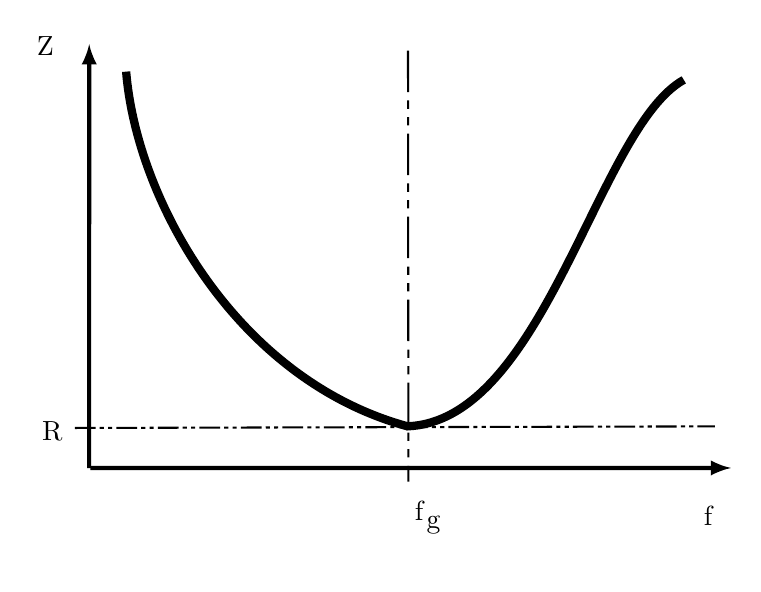
\begin{tikzpicture}
\pgftransformxscale{1.000000}
\pgftransformyscale{-1.000000}
\definecolor{dialinecolor}{rgb}{0.000000, 0.000000, 0.000000}
\pgfsetstrokecolor{dialinecolor}
\definecolor{dialinecolor}{rgb}{1.000000, 1.000000, 1.000000}
\pgfsetfillcolor{dialinecolor}
\pgfsetlinewidth{0.100000\du}
\pgfsetdash{}{0pt}
\pgfsetdash{}{0pt}
\pgfsetbuttcap
{
\definecolor{dialinecolor}{rgb}{0.000000, 0.000000, 0.000000}
\pgfsetfillcolor{dialinecolor}
% was here!!!
\pgfsetarrowsstart{latex}
\definecolor{dialinecolor}{rgb}{0.000000, 0.000000, 0.000000}
\pgfsetstrokecolor{dialinecolor}
\draw (0.005272\du,9.819848\du)--(0.002092\du,20.034838\du);
}
\pgfsetlinewidth{0.100000\du}
\pgfsetdash{}{0pt}
\pgfsetdash{}{0pt}
\pgfsetbuttcap
{
\definecolor{dialinecolor}{rgb}{0.000000, 0.000000, 0.000000}
\pgfsetfillcolor{dialinecolor}
% was here!!!
\pgfsetarrowsend{latex}
\definecolor{dialinecolor}{rgb}{0.000000, 0.000000, 0.000000}
\pgfsetstrokecolor{dialinecolor}
\draw (0.030865\du,20.029575\du)--(15.465100\du,20.028995\du);
}
% setfont left to latex
\definecolor{dialinecolor}{rgb}{0.000000, 0.000000, 0.000000}
\pgfsetstrokecolor{dialinecolor}
\node[anchor=west] at (-1.527628\du,9.872559\du){Z};
% setfont left to latex
\definecolor{dialinecolor}{rgb}{0.000000, 0.000000, 0.000000}
\pgfsetstrokecolor{dialinecolor}
\node[anchor=west] at (14.539647\du,21.180274\du){f};
\pgfsetlinewidth{0.050000\du}
\pgfsetdash{{1.000000\du}{0.200000\du}{0.200000\du}{0.200000\du}{0.200000\du}{0.200000\du}}{0cm}
\pgfsetdash{{1.000000\du}{0.200000\du}{0.200000\du}{0.200000\du}{0.200000\du}{0.200000\du}}{0cm}
\pgfsetbuttcap
{
\definecolor{dialinecolor}{rgb}{0.000000, 0.000000, 0.000000}
\pgfsetfillcolor{dialinecolor}
% was here!!!
\definecolor{dialinecolor}{rgb}{0.000000, 0.000000, 0.000000}
\pgfsetstrokecolor{dialinecolor}
\draw (7.684610\du,9.975938\du)--(7.694520\du,20.359066\du);
}
% setfont left to latex
\definecolor{dialinecolor}{rgb}{0.000000, 0.000000, 0.000000}
\pgfsetstrokecolor{dialinecolor}
\node[anchor=west] at (7.604656\du,21.062558\du){f};
% setfont left to latex
\definecolor{dialinecolor}{rgb}{0.000000, 0.000000, 0.000000}
\pgfsetstrokecolor{dialinecolor}
\node[anchor=west] at (7.604656\du,22.120892\du){};
% setfont left to latex
\definecolor{dialinecolor}{rgb}{0.000000, 0.000000, 0.000000}
\pgfsetstrokecolor{dialinecolor}
\node[anchor=west] at (7.886686\du,21.405033\du){g};
\pgfsetlinewidth{0.200000\du}
\pgfsetdash{}{0pt}
\pgfsetdash{}{0pt}
\pgfsetmiterjoin
\pgfsetbuttcap
{
\definecolor{dialinecolor}{rgb}{0.000000, 0.000000, 0.000000}
\pgfsetfillcolor{dialinecolor}
% was here!!!
\definecolor{dialinecolor}{rgb}{0.000000, 0.000000, 0.000000}
\pgfsetstrokecolor{dialinecolor}
\pgfpathmoveto{\pgfpoint{0.894716\du}{10.481474\du}}
\pgfpathcurveto{\pgfpoint{1.144716\du}{13.581474\du}}{\pgfpoint{3.564971\du}{17.920450\du}}{\pgfpoint{7.694716\du}{19.031474\du}}
\pgfusepath{stroke}
}
\pgfsetlinewidth{0.200000\du}
\pgfsetdash{}{0pt}
\pgfsetdash{}{0pt}
\pgfsetmiterjoin
\pgfsetbuttcap
{
\definecolor{dialinecolor}{rgb}{0.000000, 0.000000, 0.000000}
\pgfsetfillcolor{dialinecolor}
% was here!!!
\definecolor{dialinecolor}{rgb}{0.000000, 0.000000, 0.000000}
\pgfsetstrokecolor{dialinecolor}
\pgfpathmoveto{\pgfpoint{7.644038\du}{19.026069\du}}
\pgfpathcurveto{\pgfpoint{10.973425\du}{18.930465\du}}{\pgfpoint{12.245743\du}{11.836327\du}}{\pgfpoint{14.327718\du}{10.679675\du}}
\pgfusepath{stroke}
}
\pgfsetlinewidth{0.050000\du}
\pgfsetdash{{1.000000\du}{0.200000\du}{0.200000\du}{0.200000\du}{0.200000\du}{0.200000\du}}{0cm}
\pgfsetdash{{0.500000\du}{0.100000\du}{0.100000\du}{0.100000\du}{0.100000\du}{0.100000\du}}{0cm}
\pgfsetbuttcap
{
\definecolor{dialinecolor}{rgb}{0.000000, 0.000000, 0.000000}
\pgfsetfillcolor{dialinecolor}
% was here!!!
\definecolor{dialinecolor}{rgb}{0.000000, 0.000000, 0.000000}
\pgfsetstrokecolor{dialinecolor}
\draw (-0.342496\du,19.065408\du)--(15.079543\du,19.026853\du);
}
% setfont left to latex
\definecolor{dialinecolor}{rgb}{0.000000, 0.000000, 0.000000}
\pgfsetstrokecolor{dialinecolor}
\node[anchor=west] at (-1.377993\du,19.130129\du){R};
% setfont left to latex
\definecolor{dialinecolor}{rgb}{0.000000, 0.000000, 0.000000}
\pgfsetstrokecolor{dialinecolor}
\node[anchor=west] at (-1.446287\du,19.877398\du){};
\end{tikzpicture}

	\caption{Impedanz eines Reihenschwingkreises in Abhängigkeit von der Frequenz}
	\end{figure}
}

\subsection*{Parallelschwingkreis}

\begin{itemize}
\itemsep1pt\parskip0pt\parsep0pt
\item Baue die Schaltung des Parallelschwingkreises auf. Verwende hierfür eine Spule mit $270H$, einen $50\Omega$ Widerstand und einen $10pF$ Kondensator. 
\item Lege nun eine Wechselspannungsquelle bzw. einen Frequenzgenerator an die Schaltung an. Verwenden eine sinusförmige Wechselspannung mit einer konstanten Amplitude zwischen $1V$ und $3V$.
\item Erhöhe nun Schrittweise die die Frequenz von $1kHz$ bis $10khz$. Messen Sie für 10 Frequenzwerte den Strom der durch die Schaltung fließt.
\item Zeichne die Werte in ein Diagramm ein. Lege die Frequenz auf die X-Achse und den Strom auf die Y-Achse.
\item Was lässt sich aus dem Diagramm ablesen?
\end{itemize}

\loesung{
	\begin{figure}[H]
	\centering
	% Graphic for TeX using PGF
% Title: /media/sda2/owncloud_tu.berlin/Dia/Parallelschwingkreis_Impedanz.dia
% Creator: Dia v0.97.3
% CreationDate: Thu Nov 12 11:27:59 2015
% For: stole
% \usepackage{tikz}
% The following commands are not supported in PSTricks at present
% We define them conditionally, so when they are implemented,
% this pgf file will use them.
\ifx\du\undefined
  \newlength{\du}
\fi
\setlength{\du}{10\unitlength}
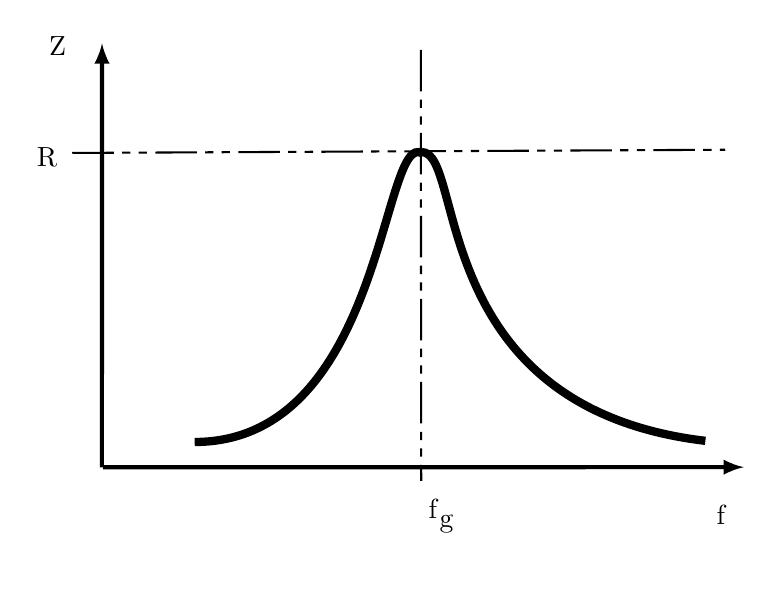
\begin{tikzpicture}
\pgftransformxscale{1.000000}
\pgftransformyscale{-1.000000}
\definecolor{dialinecolor}{rgb}{0.000000, 0.000000, 0.000000}
\pgfsetstrokecolor{dialinecolor}
\definecolor{dialinecolor}{rgb}{1.000000, 1.000000, 1.000000}
\pgfsetfillcolor{dialinecolor}
\pgfsetlinewidth{0.200000\du}
\pgfsetdash{}{0pt}
\pgfsetdash{}{0pt}
\pgfsetmiterjoin
\pgfsetbuttcap
{
\definecolor{dialinecolor}{rgb}{0.000000, 0.000000, 0.000000}
\pgfsetfillcolor{dialinecolor}
% was here!!!
\definecolor{dialinecolor}{rgb}{0.000000, 0.000000, 0.000000}
\pgfsetstrokecolor{dialinecolor}
\pgfpathmoveto{\pgfpoint{2.237980\du}{19.422900\du}}
\pgfpathcurveto{\pgfpoint{6.808680\du}{19.412500\du}}{\pgfpoint{6.737970\du}{11.870100\du}}{\pgfpoint{7.722910\du}{12.470800\du}}
\pgfusepath{stroke}
}
\pgfsetlinewidth{0.200000\du}
\pgfsetdash{}{0pt}
\pgfsetdash{}{0pt}
\pgfsetmiterjoin
\pgfsetbuttcap
{
\definecolor{dialinecolor}{rgb}{0.000000, 0.000000, 0.000000}
\pgfsetfillcolor{dialinecolor}
% was here!!!
\definecolor{dialinecolor}{rgb}{0.000000, 0.000000, 0.000000}
\pgfsetstrokecolor{dialinecolor}
\pgfpathmoveto{\pgfpoint{7.704260\du}{12.437100\du}}
\pgfpathcurveto{\pgfpoint{8.763250\du}{12.437100\du}}{\pgfpoint{7.798620\du}{18.593500\du}}{\pgfpoint{14.539600\du}{19.394800\du}}
\pgfusepath{stroke}
}
\pgfsetlinewidth{0.100000\du}
\pgfsetdash{}{0pt}
\pgfsetdash{}{0pt}
\pgfsetbuttcap
{
\definecolor{dialinecolor}{rgb}{0.000000, 0.000000, 0.000000}
\pgfsetfillcolor{dialinecolor}
% was here!!!
\pgfsetarrowsstart{latex}
\definecolor{dialinecolor}{rgb}{0.000000, 0.000000, 0.000000}
\pgfsetstrokecolor{dialinecolor}
\draw (0.005272\du,9.819850\du)--(0.002092\du,20.034800\du);
}
\pgfsetlinewidth{0.100000\du}
\pgfsetdash{}{0pt}
\pgfsetdash{}{0pt}
\pgfsetbuttcap
{
\definecolor{dialinecolor}{rgb}{0.000000, 0.000000, 0.000000}
\pgfsetfillcolor{dialinecolor}
% was here!!!
\pgfsetarrowsend{latex}
\definecolor{dialinecolor}{rgb}{0.000000, 0.000000, 0.000000}
\pgfsetstrokecolor{dialinecolor}
\draw (0.030865\du,20.029600\du)--(15.465100\du,20.029000\du);
}
% setfont left to latex
\definecolor{dialinecolor}{rgb}{0.000000, 0.000000, 0.000000}
\pgfsetstrokecolor{dialinecolor}
\node[anchor=west] at (-1.541347\du,9.891838\du){Z};
% setfont left to latex
\definecolor{dialinecolor}{rgb}{0.000000, 0.000000, 0.000000}
\pgfsetstrokecolor{dialinecolor}
\node[anchor=west] at (14.539600\du,21.180300\du){f};
\pgfsetlinewidth{0.050000\du}
\pgfsetdash{{1.000000\du}{0.200000\du}{0.200000\du}{0.200000\du}{0.200000\du}{0.200000\du}}{0cm}
\pgfsetdash{{1.000000\du}{0.200000\du}{0.200000\du}{0.200000\du}{0.200000\du}{0.200000\du}}{0cm}
\pgfsetbuttcap
{
\definecolor{dialinecolor}{rgb}{0.000000, 0.000000, 0.000000}
\pgfsetfillcolor{dialinecolor}
% was here!!!
\definecolor{dialinecolor}{rgb}{0.000000, 0.000000, 0.000000}
\pgfsetstrokecolor{dialinecolor}
\draw (7.684610\du,9.975940\du)--(7.694520\du,20.359100\du);
}
% setfont left to latex
\definecolor{dialinecolor}{rgb}{0.000000, 0.000000, 0.000000}
\pgfsetstrokecolor{dialinecolor}
\node[anchor=west] at (7.624014\du,21.027200\du){f};
% setfont left to latex
\definecolor{dialinecolor}{rgb}{0.000000, 0.000000, 0.000000}
\pgfsetstrokecolor{dialinecolor}
\node[anchor=west] at (7.624014\du,22.085533\du){};
% setfont left to latex
\definecolor{dialinecolor}{rgb}{0.000000, 0.000000, 0.000000}
\pgfsetstrokecolor{dialinecolor}
\node[anchor=west] at (7.887822\du,21.392053\du){g};
\pgfsetlinewidth{0.050000\du}
\pgfsetdash{{1.000000\du}{0.200000\du}{0.200000\du}{0.200000\du}{0.200000\du}{0.200000\du}}{0cm}
\pgfsetdash{{1.000000\du}{0.200000\du}{0.200000\du}{0.200000\du}{0.200000\du}{0.200000\du}}{0cm}
\pgfsetbuttcap
{
\definecolor{dialinecolor}{rgb}{0.000000, 0.000000, 0.000000}
\pgfsetfillcolor{dialinecolor}
% was here!!!
\definecolor{dialinecolor}{rgb}{0.000000, 0.000000, 0.000000}
\pgfsetstrokecolor{dialinecolor}
\draw (-0.712053\du,12.459658\du)--(15.018455\du,12.382548\du);
}
% setfont left to latex
\definecolor{dialinecolor}{rgb}{0.000000, 0.000000, 0.000000}
\pgfsetstrokecolor{dialinecolor}
\node[anchor=west] at (-1.810876\du,12.556046\du){R};
\end{tikzpicture}

	\caption{Impedanz eines Parallelschwingkreiseses in Abhängigkeit von der Frequenz}
	\end{figure}
}
